\documentclass{dalcsthesis}
\usepackage{fullpage}
\usepackage{textcomp}
\usepackage{graphicx}
\usepackage{algorithm}
\usepackage{algorithmic}
\usepackage{amsthm}
\newtheorem{lemma}{Lemma}

\title{Rational Secret Sharing with and without Synchronous Broadcast, Conspicuous Secrets, and Unbounded Opponents}
\author{Craig Gidney}
\date{\today}
\defenceday{1}
\defencemonth{Bla}
\defenceyear{3023}

\begin{document}
\mcs
\maketitle

\chapter{Introduction}

Secret sharing allows some data $s$ to be split into $n$ shares such that any set of $t$-1 shares reveal no information about $s$ but any set of $t$ shares can be used to easily compute $s$. Shamir [REF] elegantly solved this problem in 1974. However, recent interest has focused on the practical issues of recombining shares of a secret in the presence of adversarial players.

This paper presents protocols and bounds on the effectiveness of any protocol for recombining secrets in the presence of players who do not want others to learn the secret (rationality), may not want to learn the secret themselves (maliciousness), may be colluding, may have unbounded computational capacity, may not be able to synchronize sends (synchronous broadcast), and/or may be able to recognize the secret independently (conspicuousness).

[map of the rest of document]

\chapter{Properties and Definitions}

Several properties and definitions are important to understand the rest of this paper.

\section{Rational Players}

Rational players want to learn the secret but secondarily want to prevent other players from learning the secret. They must be incentivized into cooperating by ensuring it always results in a higher probability of learning the secret.

Rationality is a far more practical assumption than honesty, because most real world actors are rational. For example, consider a group of financial firms with shares to valuable market information. Each firm would profit from access to the information, but would profit even more from exclusive access. They want the secret but also don't want others to have the secret. They are rational players.

After a rational player learns the secret, they effectively become malicious.

\section{Malicious Players}

Malicious players only care about preventing other players from learning the secret. They want the process of learning the secret to be delayed, aborted, and corrupted. They can't be incentivized into cooperating. Instead, their actions must be authenticated and constrained.

Even a few unchecked malicious players can create huge search spaces. If 10 out of 100 shares are faked, the probability of choosing a subset of 80 authentic shares is about $3.4 * 10^{-16}$. Without some method to reduce the search space it could take centuries of millions of attempts per second to find a valid subset.

\section{Coalitions}

Coalitions are groups of players working together to further their goals. Good protocols must minimize or eliminate the benefits of forming a coalition.

Coalitions of rational players can have up to $t-1$ members. Larger rational coalitions exceed the threshold to learn the secret and become malicious. Coalitions of malicious players can have up to $n-1$ members. Malicious coalitions with more than $n-t$ players can trivially prevent the secret from being learned, but may attempt to go further and cause the wrong secret to be learned.

\section{Interactive Dealer}

Several papers assume the dealer is available to re-issue shares of the secret on demand. This assumption simplifies the problem considerably. In fact, if the dealer is not limited to just re-issuing shares, the problem becomes trivial: the dealer accepts votes to reveal the secret and does so when the number of votes exceeds the threshold.

Note that a dealer with the ability to generate shares but the inability to count votes is not necessarily absurd. The dealer may be a simulation within a multi party computation, with restrictions on possible computation due to security or performance concerns.

All the results in this paper assume a non-interactive dealer.

\section{Honest Dealer}

The nature of secret sharing gives the dealer significant power. Nothing within the protocol can prevent the dealer from encoding the wrong secret or giving a player extra information. But there are other ways the dealer can misbehave and failing to detect or curb those behaviours is assuming an honest dealer.

For example, if a protocol requires a sacrifical player to not learn the secret then the dealer may always choose the same player as the sacrifice. Another example is the dealer failing to ensure a protocol's termination condition occurs, leaving the players to waste time executing the protocol.

The protocols in this paper will assume the dealer is honest, but do not have to. The following two methods, where applicable, fix the assumption:

\begin{itemize}
  \item The dealer commits to the shares but before shares are distributed the players shuffle the share-to-player mapping. This prevents the dealer from biasing the protocol against a chosen subset of players.
  \item The dealer commits to shares of a random secret but before shares are distributed the players choose to either check or accept. If they choose to check then the dealer reveals the entropy used to generate the shares, the players verify they were generated correctly from the given entropy, and the process repeats. If they choose the check then the dealer distributes the shares and reveals the offset from the shared secret to the true secret. This prevents the dealer from undetectably creating invalid or malformed shares.
\end{itemize} 

\section{Synchronous Broadcast}

Synchronous broadcast is the ability for players to send their message (or commit to not sending a message) for a round before being able to receive any other player's message(s) for that round. Without synchronous broadcast, message orderings must be explicit. Two rational players exchanging messages without a specified order will deadlock because they both have an incentive to wait to receive before deciding to send.

This paper explores the consequences of losing synchronous broadcast. We generalize synchronous broadcast to k-broadcast (allowing up to k players to perform a synchronous broadcast), with $n$-broadcast and $1$-broadcast corresponding to fully synchronous and asynchronous broadcast respectively. However, we still assume the same message is reliably sent to all players, meaning two receivers will not disagree about receiving a message or the received message's content.

\section{Unbounded Players}

Unbounded players can perform any desired finite number of computations within a fixed time. They can trivially break schemes relying on computational difficulty, like reversing one way functions, but can't defeat schemes secure in the information theoretic sense, like encryption with a one-time-pad or Shamir's Secret Sharing Scheme.

This paper proposes protocols for both bounded and unbounded players. Protocols that work in the presence of unbounded players are secure in a much stronger sense, but can't rely on tools like secure pseudo random number generators.

\section{Conspicuousness of the Secret} 

A secret is conspicuous if, given a guess at the secret, it is possible to determine if the guess is the secret. For example, the combination to a lock is conspicuous because, given a combination, you can check if it works. On the other hand, the combination to a 'burn safe', which destroys itself and its contents if the wrong combination is entered, is effectively inconspicuous.

Any secret can be made conspicuous using a bit commitment, but returning to inconspicuousness is impossible. However, conspicuousness is a tradeoff. It prevents the wrong secret from being accepted but allows unbounded opponents to brute force the secret and, as shown later, requires a player to be sacrificed if communication is asynchronous.

Conspicuousness can be relative to the player or group of players. A secret may be conspicuous to one player but not another or to a pair of players but neither individually. Once a secret sharing protocol starts the secret must be at least conspicuous to groups of players over the threshold size, because they can compute the secret. This paper, when refering to conspicuousness, will implicitely be refering to the original conspicuousness of the secret, before the protocol started, unless otherwise noted. Protocols for inconspicuous secrets are not required to maintain the inconspicuousness of the secret.

\chapter{Previous Work}

In 1979 Adi Shamir published the paper [How to Share a Secret], detailing how to divide a secret into $n$ shares with a threshold $t$ such that any set of $t$ shares can easily reconstruct the secret but fewer than $t$ shares provided no information about the secret. In Shamir's scheme, shares are points on an up-to-$(t-1)$'th degree polynomial over a finite field of size $p$. The secret is the polynomial's value at $x=0$. An up-to-$(t-1)$'th degree polynomial can be interpolated from any set of $t$ points but with only $t-1$ points there is exactly one matching polynomial for each possible value at $x=0$. The final share can cause the secret to be any value. Thus an attacker with $t-1$ shares has no more information about the secret than an attacker with $0$ shares. The scheme is secure in the information theoretic sense.

The rational secret sharing problem was introduced by Halpern and Teague in their paper [Rational Secret Sharing and Multiparty Computation]. They showed that, if all players are rational, prefering to learn the secret but secondarily prefering others to not learn the secret, then there is no protocol with bounded worst-case completion time (because not sending on the last round is weakly dominant and rational players will backwards induct this dominance all the way to the first round). They then provided a randomized round-based protocol with bounded expected time. Each round is either a check round or the final round, and this fact can only be determined after the round has occured. Rational players cooperate because defecting in check rounds results in not learning the secret.

In the paper [Games For Exchanging Information] Kol and Naor present two protocols for rational non-malicious non-colluding players with synchronous broadcast and an inconspicuous secret. They avoid cryptographic primitives, like one way functions, arguing that they implicitely bound the number of rounds and thus cause rational players to defect. As a result, their protocol does not rely on computational difficulty and works equally well for unbounded players.

The first protocol is for the 2-of-2 case. The dealer generates a short list of random entries with geometric distributed length and a long list starting with the short list, followed by the secret, and then random entries with a geometric-distributed length. Each round players send the next entry in their list. If the sent values do not match, the protocol is aborted. If one player does not send a value, it is assumed they were the short player and the single sent value is the secret.

The second protocol is for the general $t$-of-$n$ case. In this augmented protocol every player but one gets the long list, list entries include authentication information as well as $t$-of-$n$ shares of an 'indicator' flag which allows subsets without the short list to notice the final round, and future list entries must be unmasked using shared information from previous rounds.

As remarked in the paper, Kol and Naor's generalized protocol is susceptible to coalitions. If a coalition includes the short player then they know the last round and can betray the other players. If the coalition does not include the short player then they know a slightly stricter upper bound on the final round, allowing them to stay silent on the final round when the long lists have minimum length.

Kol and Naor also note that their 2-of-2 protocol is not dependent on synchronous broadcast, as long as the dealer predefines the order messages must be sent and includes authentication. The long player sends first on the definitive round, which the short player knows but can't hide because they have no authenticated messages for that round. The short player learns the secret from the long player sending, and the long player learns they sent the secret from the short player no sending.

[This paper's synchronous protocol for unbounded opponents is based on Kol and Noar's protocols. But they are extended to work against malicious and rational opponents.]

Other papers on rational secret sharing include:

\begin{itemize}
  \item Fairness with an Honest Minority and a Rational Majority by Shien Jin Ong, David  C. Parkes, Alon Rosen, and Salil Vadhan
    \subitem Proposes a single-round asynchronous protocol that works probabilistically if some players are honest. Rational players are incentivized to cooperate by the likelihood of an honest player reciprocating.
  \item Rational Secret Sharing with Repeated Games by Shaik Maleka, Amjed Shareef, and C. Pandu Rangan
    \subitem Proposes an asynchronous protocol requiring an interactive dealer.
  \item Collusion Free Protocol for Rational Secret Sharing by Amjed Shareef
    \subitem Extends Kol and Naor's protocol to be more resilient to coalitions when the threshold is not a majority.
  \item paper using homomorphic encryption to emulate ack-ing\ldots
    \subitem Very expensive. Implementation details very complicated? Relies on multi party computation (is secret sharing supposed to enable more efficient multi party computation?).
\end{itemize}

\chapter{Used Cryptographic Systems}

Generator/Verifier (Pedagogical Example: RSA)

- Generator takes a nonce and outputs a secure value
- Verifier accepts value/nonce pairs and determines if they came from the generator
- Verifier can't be used to efficiently generate matching pairs

Bit commitment:

- Salted hash
- Implied by Generator/Verifier

Secure Secret Sharing Scheme (without sharing protocol) (Example: Shamir's)

- Fewer than M shares provides no information about secret
- At least M shares provide complete information about secret

Secure Pseudo Random Number Generator (Pedagogical Example: Blum Blum Shub)

- No efficient algorithm to distinguish output from random

Bit Commitment

Verifiable Random Function (VRF)

A VRF produces secure pseudo random values alongside proofs that the values were correctly generated. VRFs were introduced by [Verifiable Random Functions by Silvio Micali, Michael Rabiny, Salil Vadhanz], and a more efficient implementation can be found in [A Verifiable Random Function with Short Proofs and Keys by Yevgeniy Do dis, Aleksandr Yampolskiy]. This paper will use plain RSA as an example VRF because of its simplicity, even though such usage actually compromises RSA's security. Thus it will be referred to as 'Pedagogical RSA VRF'. In Pedagogical RSA VRF inputs are encrypted with the private key to create verifiable random values, no additional proof information is attached, and verifiable random values are checked by ensuring they decrypt to the expected input.  

\chapter{Synchronous Broadcast}

[PREAMBLE]

\section{Optimal Synchronous Protocol for Bounded Opponents}

The easiest case for rational secret sharing is when synchronous broadcast is present and opponents are not computationally unbounded. When both these assumptions are given the secret can be made conspicuous without cost, allowing a simpler protocol.

The protocol proposed here is optimal in terms of resilience against coalitions. Rational coalitions up to size $t-1$ gain no advantage. Malicious coalitions up to size $n-t$ gain no advantage. Malicious coalitions up to size $n-1$ can't convince players to accept the wrong secret. These bounds are a consequence of the nature of secret sharing and hold for any protocol.

At a high level, the protocol works as follows. Each round every player sends a message created by a verifiable random function (VRF) provided by the dealer. The messages are added to offsets also provided by the dealer. Before the target round the round shares (the messages plus their offsets) are uncorrelated, but the dealer chooses the offsets such that on the target round the round shares form a valid set of $t$ of $n$ Shamir shares for the secret. Players recognize the target round, after it occurs, by noticing that the round shares combined into a value matching a bit commitment to the secret provided by the dealer.

\begin{algorithm}
  \caption{Synchronous Dealer Protocol for Bounded Opponents}
  \label{alg:SB_Dealer}
  \begin{algorithmic}[1]
    \INPUT Prime $p$ larger than the largest possible message
    \INPUT Total number of shares $n$
    \INPUT Threshold number of shares $t$
    \INPUT Marginal probability of target round occuring $\lambda$
    \INPUT Verifying function scheme $VRFS$
    \INPUT Commitment scheme $CS$
    \INPUT Secret natural number $s$ less than $p$
    \OUTPUT $n$ shares
    \STATE Create a commitment $c$ to the secret $s$
    \STATE Create $n$ public/private key pair $V_i, G_i = VRFS.Create()$
    \STATE Pick the target round $r$ using a geometric distribution with marginal probability $\lambda$
    \STATE Create $n$ Shamir shares $S$ for the secret with a threshold of $t$
    \STATE Compute the $n$ share/message offsets $F_i = S_i - VRF(G_i, r).Value$
    \STATE Create the common share composed of all public keys $V$, offsets $F$, and the commitment $c$
    \STATE Return the $n$ shares composed of the common share, index $i$, and private key $G_i$
  \end{algorithmic}
\end{algorithm}
\begin{algorithm}
  \caption{Synchronous Player Protocol for Bounded Opponents}
  \label{alg:SB_Player}
  \begin{algorithmic}[1]
    \INPUT Prime $p$ larger than the largest possible message
    \INPUT Total number of shares $n$
    \INPUT Threshold number of shares $t$
    \INPUT Verifying function scheme $VRFS$
    \INPUT Commitment scheme $CS$
    \INPUT Player Index $i$
    \INPUT VRFS Private Key $g$
    \INPUT $n$ VRFS Public Keys $V$
    \INPUT $n$ Shamir Share Offsets $F$
    \INPUT Secret Commitment $c$
    \INPUT Synchronous Network $NS$
    \OUTPUT Secret value $s$ or failure
    \FOR { each round $r$ }
      \STATE Send the round message $M_{i,r} = VRFS.Generate(g, r)$ to all cooperating players
      \STATE Receive round messages $M_{j,r}$ from other players
      \STATE Mark players that sent no message as non-cooperating
      \STATE Discard any messages that do not verify $VRFS.Verify(V_j, M_{j,r})$
      \STATE Mark players that sent invalid message as non-cooperating
      \STATE Use known messages to compute the known round shares $S_{j,r} = M_{j,r}.Value + F_j$
      \STATE If the number of known round shares is less than $t$ then return Failure
      \STATE Combine any $t$ of the known round shares to get a potential round secret $X_r$
      \STATE If the secret matches the commitment $CS.Matches(c, X_r)$ then return $X_r$
    \ENDFOR
  \end{algorithmic}
\end{algorithm}

\begin{figure}
  \caption{Example run of synchronous bounded protocol}
  \label{Ex:SB}
  \begin{itemize}
    \setlength{\itemsep}{0pt}
    \setlength{\parsep}{0pt}
    \setlength{\parskip}{0pt}
    \item Parameters
    \subitem Finite Field Size $p = 5$
    \subitem Share Count $n = 2$
    \subitem Threshold $t = 2$
    \subitem Verifiable Random Functions $PedagogicalRSA(p: 7, q: 11)$
    \subitem Commitment Scheme $CS = PlainSHA1$
    \subitem Secret $s = 3$
    \item Dealing
    \subitem Create commitment $c = CS.Create(s) = 0x984292\ldots$
    \subitem Create RSA key pairs for VRFS
    \subsubitem $G_1, V_1 = 53, 17$
    \subsubitem $G_2, V_2 = 37, 13$
    \subitem Pick the target round $r = 3$
    \subitem Create shamir shares
    \subsubitem $P(x) = 3 + 4x \pmod{5}$
    \subsubitem $S_1 = (1, 2)$, $S_2 = (2, 1)$
    \subitem Compute the offsets 
    \subsubitem $F_1 = 2 - (3^{53} \pmod{77}) \pmod{5} = 2$
    \subsubitem $F_2 = 1 - (3^{37} \pmod{77}) \pmod{5} = 0$
	\item Round 1
	\subitem Player 1 send $1^{53} = 1$
	\subitem Player 2 sends $1^{37} = 1$
	\subitem Players verify $1^{13} = 1$ and $1^{17} = 1$
	\subitem Round shares are $P(1) = 1+2 = 3$, $P(2) = 1+0 = 1$
	\subitem Round polynomial $P(x) = 0 + 3x \pmod{5}$ gives secret $P(0) = 0$
	\subitem Continue because $\not CS.Matches(0, c)$
	\item Round 2
	\subitem Player 1 send $2^{53} = 74 \pmod{77}$
	\subitem Player 2 sends $2^{37} = 51 \pmod{77}$
	\subitem Players verifiy $51^{13} = 2 \pmod{77}$ and $74^{17} = 2 \pmod{77}$
	\subitem Round shares are $P(1) = 74+2 = 1$, $P(2) = 51+0 = 1$
	\subitem Round polynomial $P(x) = 1 + 0x \pmod{5}$ gives secret $P(0) = 1$
	\subitem Continue because $\not CS.Matches(1, c)$
	\item Round 3
	\subitem Player 1 send $3^{53} = 5 \pmod{77}$
	\subitem Player 2 sends $3^{37} (mod 77) = 31 \pmod{77}$
	\subitem Players verify $31^{13} = 3 \pmod{77}$ and $5^{17} = 3 \pmod{77}$
	\subitem Round shares are $P(1) = 5+2 = 2$, $P(2) = 31+0 = 1$ 
	\subitem Round polynomial $P(x) = 3+4x \pmod{5}$ gives secret $P(0) = 3$
	\subitem Succeed with 3 because $CS.Matches(3, c)$
  \end{itemize}
\end{figure}

In additional to being optimal against coalitions, this protocol has relatively low computational costs. Both the dealer and player protocol's costs are dominated by evaluating and verifying the output of verifiable random functions. Failing to authenticate messages makes malicious players stronger. Reducing the number of messages makes both types of coalition stronger. It's not clear how the efficiency can be improved without sacrificing security.

\begin{lemma} Malicious players and coalitions will defect \end{lemma}
\begin{proof}
The conspicuousness of the secret and verification of messages places severe constraints on player actions. Cooperating and sending the correct messages can only increase the probability of other players learning the secret.

Malicious players and coalitions will always want to defect before the target round occurs. They defect by sending a random message, instead of no message, because of the negligible but non-zero chance of passing verification. If possible they will wait to defect on the target round because forging a message on that round stops the protocol from terminating deterministically.

Players and coalitions with size less than $t$ will defect immediately, because they can't determine if the next round is the target round or not. Coalitions with size at least $t$ can predict the target round and defect at that time. But ultimately their chances of success are negligible and easily reduced, so we can make the simplifying assumption that they send no messages (they 'drop').
\end{proof}

\begin{lemma} Cooperation is a Nash equilibrium for rational coalitions and players \end{lemma}
\begin{proof}
Let $C$ be a rational coalition of between $1$ and $t-1$ (inclusive) rational players. Larger coalitions are not rational because they learn the secret and become malicious. $|C| = 1$ corresponds to a non-colluding rational player.

All other players are either malicious or rational. Malicious player will defect immediately. In order to show cooperation is a nash equilibrium, assume the other rational players are cooperative. They follow the protocol correctly until the secret is learned or there are fewer than $t$ players who have not defected remaining.

Let the number of malicious players be $m$. Assume without loss of generality that $n - m >= t$, since otherwise no one will learn the secret and all strategies have equivalent outcomes. Assume without loss of generality that $n - m - |C| < t$, since otherwise the coalition can't prevent others from learning the secret and has no incentive to defect.

Each of the colluders within the coalition can cooperate or defect. Let $d$ be the number of colluders who must defect to cause the number of players who have not defected to drop below $t$. Let 'crossing the threshold' mean the number of colluders becomes larger than $d$ for the first time. Crossing the threshold prevents other players from learning the secret but also causes the rational players to stop participating. Crossing the threshold before the target round results in the coalition not learning the secret. Failing to cross the threshold on the target round results in all rational players learning the secret.

The coalition can't recognize the target round until after it occurs. They need at least $t$ shares to create the round secret, allowing a comparison against the commitment, but they have at most $t-1$ shares. Instead, every round the coalition knows only that there is a $\lambda$ probability of it being the target round.

Given the coalition's probabilistic knowledge of the target round, it can compute the expected payoff of crossing threshold. Doing so this round gives a $\lambda$ chance of learning the secret while preventing others from learning the secret, but a $1-\lambda$ chance of not learning the secret. Crossing the threshold next round result in a $\lambda + (1-\lambda)*\lambda$ chance of learning the secret, a $(1-\lambda)*\lambda$ chance of others not learning the secret, and a $(1-\lambda)^2$ chance of not learning the secret.

The expected payoff of crossing the threshold next round instead of this round is higher. The coalition will always want to cross the threshold later instead of now. Therefore the coalition never wants to cross the threshold. The only time a colluder will defect is when they know doing so will not cross the threshold.

Crossing the threshold is the only way to prevent other players from learning the secret but the coalition rationally chooses not to do so. Therefore all rational players, including the coalition, will learn the secret. This is the same payoff achieved by the assumed equilibrium strategy. Therefore cooperating is a weak nash equilibrium.

Cooperating is also a strong nash equilibrium, but only if there may be enough malicious players that even one colluder defecting can result in the coalition not learning the secret.
\end{proof}

Note that other, less ideal, strategies are also nash equilibriums under the assumption that all players are malicious or rational. For example, 'everyone defect on round 3' is a nash equilibrium. But if there is the possibility of honest players, who initially cooperate but still punish defectors, then only the cooperative strategy is an equilibrium.

\section{Synchronous Protocol for Inconspicuous Secrets allowing Unbounded Opponents}

When opponents are computationally unbounded they have the ability to brute force many cryptographic primitives. Any primitive that is not secure in the information theoretic sense needs to be replaced by one that is. As a consequence, the protocol will require significantly more entropy.

Our goal is to bound the amount of knowledge opponents have about the secret. The most important consideration for bounding their knowledge is the likelihood of terminal messages. A terminal message or message set is a message which, if received, will cause the player to accept a specific secret. The more likely a terminal message is, the more knowledge the opponent has about the secret. Decreasing the probability of individual terminal messages decreases the amount of knowledge opponents have about the secret, but also necessarily increases the expected number of rounds or the amount of entropy in messages.

\subsection{Replacing Verifiable Random Functions with Points on Lines}

Unbounded opponents can brute force VRFs, so a different message verification scheme is needed. We want to create a signed message for the sender and a verifier for each receiver. Each verifier must be able to detect forged messages with high probability, even if the sender colludes with other verifier. Verifiers should not be able to predict the message, even when colluding.

There is a simple system satisfying these necessary properties. Sign the message by transforming it into the slope of a line with random offset in a finite field. Give the verifier a random point on the line. Use a new random line and point for each verifier.

The sender can't forge messages because changing the message means changing the slope of the line and picking a new offset. But each possible new line only intersects the old line at one point. If the verifier's point is not at that point, which is more likely the larger the finite field is, the forgery is detected.

The verifier can't determine the expected message because for each possible slope, corresponding to a message, there is an offset that causes the line to pass through the check point. The verifier only knows how the slope relates to the offset, not the slope or offset individually.

Verifiers can't collude to learn the message slope and the sender can't collude with verifiers to fool other verifiers because each check point is for an independent line.

[REF was mentioend in some paper look that up]

\begin{algorithm}
  \caption{Create a Verifiable Message for an Unbounded Opponent}
  \label{alg:CreatingVerifiableMessageForUnbounded}
  \begin{algorithmic}[1]
    \INPUT Prime $p$ larger than any possible message
    \INPUT Message $m$
    \OUTPUT A signed message $m$, $b$ and a verifier $v_x$, $v_y$
    \STATE Let $b$ be a random natural number below $p$ 
    \STATE Let $v_x$ be a random natural number below $p$
    \STATE Let $v_y = b + m*v_x \pmod{p}$
    \STATE Return $m$, $b$, $v_x$, $v_y$
  \end{algorithmic}
\end{algorithm}

\begin{figure}
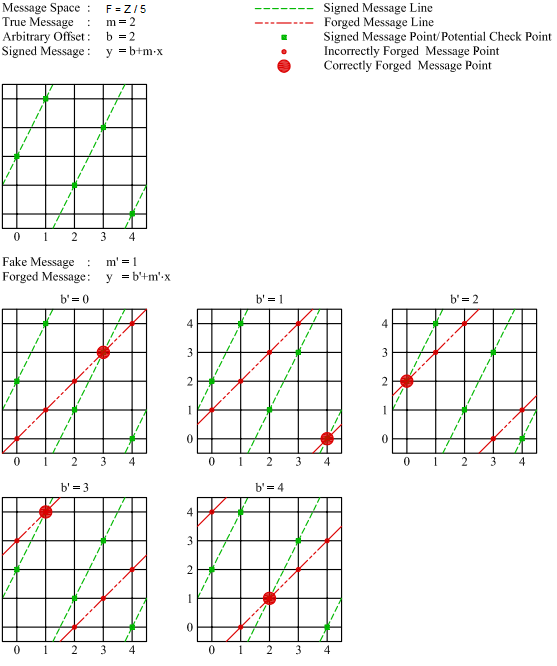
\includegraphics[width=\textwidth]{../../Graphics/PointAndLineExample.png}
\caption{Changing a signed message requires choosing an offset corresponding to an unknown check point. Chance of successful forging: $\frac{1}{p}$.}
\label{img:ForgingVerifiableMessageForUnbounded}
\end{figure}

\subsection{Overview}

The dealer will give each player a list of messages to send, one per round. Specifying the messages exactly is necessary because messages need high marginal entropy. If players derived multiple messages from small amounts of information, it is possible for unbounded opponents to make reasonable guesses at the secret's value before the protocol ends. We want to maintain a security factor on the order of $\frac{1}{p}$, so each message will have at least $p$ possibilities. Of course, messages are augmented with verification information to prevent forgery.

Because players are receiving a finite list of messages, they each know an upper bound on the number of rounds based on the length of their list. The protocol must end as the shortest list ends, or else the player with the shortest list will be excluded from the result. Care has to be taken to ensure players continue to cooperate even as their list ends, or else not sending will be weakly dominant and rational players will drop.

Each round of messages will combine to form a potential secret. Determining if the potential secret is the true secret has to be done carefully, because cryptographic primitives like bit commitment with one way functions don't work against unbounded opponents. We will use additional 'indicator' shares which, when they all come up 0, indicate the potential secret is the true secret. Each message will be composed of one secret share and several indicator shares (the necessary number depends on the threshold and number of players). Note that the message verification can be done per-share-in-the-message instead of per-message (convenient because shamir shares are already members of a finite field with prime size). 

The last round can occur before the shortest list ends (the normal case) or the round after the shortest list ends (the short case). In the short case, the short player will send no message on the final round despite being present. But the remaining players must be able to distinguish a player dropping due to the short case and a player dropping for other reasons. For this purpose, an additional 'short share' is given to all players. The short share is used to replace the missing share when the number of players drops from $t$ to $t-1$. The short share has no verification information and is masked with the previous message from the short player. This prevents it from being used when the short player is not present and prevents players from identifying the short player before the final round by noticing the verification information will match. Instead of verification information, the short share relies on the indicators being non-zero to prevent a random secret from being accepted.

\begin{algorithm}
  \caption{Synchronous Dealer Protocol for Unbounded Opponents and Inconspicuous Secrets}
  \label{alg:SB_Dealer}
  \begin{algorithmic}[1]
    \INPUT Prime $p$ larger than the largest possible message
    \INPUT Total number of shares $n$
    \INPUT Threshold number of shares $t$
    \INPUT Marginal probability of target round occuring $\lambda$
    \INPUT Minimum message list size $\beta$
    \INPUT Secret natural number $s$ less than $p$
    \OUTPUT $n$ shares
    \STATE Let the number of indicators be (at least) $i = 2 + (log_m {n \choose t}*t)$
    \STATE Generate the $n$ random length differences for the lists: $d_x = Geometric(stopChance: sqrt(\alpha))$
    \STATE Compute the list lengths: $L_1 = \beta + d_1, L_x = L_{x-1} + 1 + d_x$
    \STATE Choose a target round $r$ from a geometric distribution with marginal stop chance $\alpha$. This must be done carefully, because $r$ is bounded by the shortest list length. To keep $r$'s distribution correct use marginal stop chance of $\alpha$ until round $\beta$ then a marginal stop change of $sqrt(\alpha)$ until the end of the shortest list then stop. Combining the distribution of the end of the shortest list with this modified distribution for $r$ results in the overall correct distribution for $r$.
    \STATE Generate Shamir shares for round secrets $S_{round}^{player}$ for each round up to $L_{n}$. The secret is random, except on the target round when it is the desired secret.
    \STATE Generate Shamir shares for indicators $I_{round,iundex}^{player}$ for each indicator and round up to $L_{n}$. The indicator values are random non-zero for every round except the target round, when they are all zero.
    \STATE Sign every secret and indicator share for every receiving player.
    \STATE Compute the short shares for the secret and indicators: $S_{short} = S_r^1 - S_{r-1}^1, \forall x . I_{short,x} = I_{r,x}^1 - I_{r-1,x}^1 \pmod{p}$
    \STATE Shuffle the list lengths.
    \STATE Return the $n$ shares composed of the player index $i$, short share, a list of signed secret and indicator shares, and lists of verifiers for expected secret and indicator shares (all lists are trimmed to contain $L_i$ items).
  \end{algorithmic}
\end{algorithm}
\begin{algorithm}
  \caption{Synchronous Player Protocol for Unbounded Opponents and Inconspicuous Secrets}
  \label{alg:SUI_Player}
  \begin{algorithmic}[1]
    \INPUT Prime $p$ larger than the largest possible message
    \INPUT Total number of shares $n$
    \INPUT Threshold number of shares $t$
    \INPUT Player Index $i$
    \INPUT List of $r_{ceil}$ signed secret shares $S$
    \INPUT List of $r_{ceil}$ arrays of signed indicator shares $I$
    \INPUT List of $r_{ceil}$ verifiers for remote signed secret and indicator shares
    \INPUT Synchronous Network $NS$
    \OUTPUT Secret value $s$ or failure
    \FOR { each round $r$ satisfying $1 <= r <= r_{ceil} + 1$}
      \STATE Let $c_1$ be the number of players who have not been marked as non-cooperating (including us)
      \IF {$c_1 < t$}
      	\STATE Return Failure
      \ENDIF
      \IF { $r > r_{ceil}$ }
      	\STATE Send no messages
      \ELSE
      	\STATE Send signed secret and indicator shares from lists for this round
      \ENDIF
      \STATE Receive signed secret and indicator shares from other players
      \STATE Mark players that sent no message or messages with incorrect signatures as non-cooperating
      \STATE Discard messages from non-cooperating players
      \STATE Let $c_2$ be the number of players who have now not been marked as non-cooperating (including us)
      \IF {$c_2 < t - 1$}
      	\STATE Return Failure
      \ELSIF {$c_2 = t - 1$}
        \IF {$r <= r_{ceil}$}
          \STATE Return Failure
          \FOR {each player $x$ who sent no message for the first time this round}
            \STATE Offset the short share components with $x$'s components from the previous round to get the final share components
            \STATE Combine the available shares and the final share to get the indicators and round secret
            \IF {all indicators are zero}
              \STATE Return the round secret 
            \ENDIF
          \ENDFOR
        \ENDIF
      \ELSE
        \IF { $r > r_{ceil}$}
          \STATE Offset the short share components with our previous share components to get our share for this round
        \ENDIF
        \STATE Combine the available shares to get the indicators and round secret
        \IF {all indicators are zero}
          \STATE Return the round secret 
        \ENDIF
      \ENDIF
    \ENDFOR
    \STATE Return Failure
  \end{algorithmic}
\end{algorithm}

\section{Rational players play honestly}

Note: A rational player with a larger list will cooperate for at least as many rounds as a rational player with a smaller list. Otherwise the player with a larger list could simulate having a smaller list and do better, contradicting their rationality.

Proof by induction: Rational players with lists of length up to $f$ will play honestly.

There is a shortest possible list length $\beta$.

Base case: suppose a player $e$ has a list with the shortest possible length $f = \beta$. $e$ knows the final round is, at the lastest, round $f+1$. $e$ also knows other rational players, having larger lists, will cooperate for at least as many rounds as $e$. In order to reach round $f+1$, which could occur, $e$ must cooperate every round until after round $f$. On round $f+1$, $e$ will not send any messages (and can't send any messages with forging), but is compensated for by the short share and has thus cooperated. Therefore a player with the shortest possible list length will play honestly.

Inductive case: Suppose a player $x$ has a list of length $f > \beta$. $x$ knows, by induction, that players with shorter lists will player honestly. $x$ also knows that players with longer lists will cooperate for at least as many rounds as $x$ cooperates. $x$ knows the final round is, at the latest, round $f+1$. $x$ must cooperate every round until round $f$ has finished to have the chance to reach round $f+1$. If we reach round $f+1$, $x$ will not send any messages (and can't send any messages with forging), but is compensated for by the short share and has thus cooperated. Therefore $x$ will play honestly.

QED.

\section{In the short case, coalitions with $t-1$ members can detect the final round before it occurs, but this can be made negligible by increasing $\beta$}

Let $C$ be a coalition with $t-1$ members. Let $d$ be the short player. Let $r$ be the final round and assume it occured due to $d$'s list running out. Either $d \in C$ or $d \notin C$. If $d \in C$ then after round $r-1$ the coalition knows $d$'s list has run out and thus knows $r$ is the final round. If $d \notin C$ then after each round the coalition can simulate each of the non-coalition players, including $d$, dropping. After round $r-1$, this simulation will determine that $d$ is the short player and round $r$ is the final round.

Note that normal-case final rounds can't be detected in this way. An easy way to make this attack negligible is by increasing $\beta$. If we want a security factor of $m$ and our round finish probability is $\alpha$ then we must satisfy $(1 - \alpha)^\beta <= 1/m$. Solving for $\beta$ gives $\beta >= \frac{log(m)}{-log(1 - \alpha)}$

\section{Malicious coalitions have many chances to inject a false secret by using the drop share, but this can be made negligible by increasing $i$}

Opponents with unbounded computational resources can search for attacks much more effectively. All messages in this protocol, except the short share, are protected from brute force using the line-point verification system. Thus we can limit our analysis to how the short share can be abused.

The short share comes into effect when at least $t$ players sent valid messages in the previous round but only $t-1$ sent valid messages this round. This occurs by design in the short case, but also occurs when players drop for other reason. In particular, malicious players have some control over triggering the short share. In the worst case, there will be $n-1$ malicious players and 1 honest player. The malicious players can easily prevent the honest player from learning the secret but they also have a chance to cause them to learn the wrong secret. The result of using the short share varies based on the remaining players, the short player, and the round, so the malicious players have ${n-1 \choose t-1}*(t-1)*r$ chances. Each chance will generate an effectively random secret and set of indicators. If there are too few indicators, it is almost certain that there will be some place the short share can cause an incorrect secret to be accepted. Since the malicious players are unbounded, they can easily find any such case.

To prevent this case from occuring, we must choose the number of indicators wisely. Since the size of our secret space is $m$, and we can easily achieve that security factory, that will be the goal. There is a $\frac{1}{m^i}$ chance of $i$ indicators coming up 0. The malicious players have at most ${n-1 \choose t-1}*(t-1)*r$ independent chances. Their total probability of success is less than $\frac{{n \choose t}*t*r}{m^i}$. Thus we solve $\frac{{n \choose t}*t*r}{m^i} < \frac{1}{m}$ for $i$ and get $i > log_m {n \choose t}*t*r*m = 1 + (log_m r) + (log_m {n \choose t}*t)$. Since $r$ is a random variable and we must pick $i$ before $r$, we need to choose a reasonable upper bound. $r <= m$ is extremely likely, since $m$ is very large, and will easily fit within our security factor. Therefore setting $i = 2 + log_m {n \choose t}*t$ is sufficient to prevent malicious players from misusing the short share with high probability.

\chapter{Asynchronous Broadcast}

Communication is inherently asynchronous. The primary limitation of the preceding protocol is its reliance on synchronous broadcast. Without the synchronization, rational players following the protocol would deadlock by trying to get an advantage by waiting for each others' messages before sending. Unfortunately, synchronous sending is not a very practical assumption. For example, messages sent over the internet are inherently asynchronous.

This section explores the consequences of losing synchronous broadcast by generalizing it to partially synchronous broadcast. In partially synchronous broadcast, up to $p$ messages can be sent synchronously. Asynchronous broadcast corresponds to $p=1$ and synchronous broadcast corresponds to $p=n$.

\section{Lemma: For any protocol where all players are rational, the secret is conspicuous and communication is asynchronous, at least one player will not learn the secret}

We will prove this result by contradition. Assume all players learn the secret.

Let $r$ be the first round such that, at the end of round $r$, all players know the secret. Let $L$ be the set of players who learn the secret during round $r$. Let $s$ be the expected sender of round $r$'s message. Let $m$ be the message, or lack of a message, sent in round $r$.

$m$ is a message, not the lack of a message. Because the secret is conspicous, players can attempt to brute force it by pre-emptively trying likely messages. The easiest possibility to try is the lack of a message. If $m$ was the lack of a message, then the memberes of $L$ would have tried this possibility at the end of the previous round and learned the secret before round $r$. If $m$ is the lack of a message then $r$ is not the first round a player learns the secret, contradicting our assumptions.

$s \in L$. If $s$ knew the secret before round $r$, then $s$ would have sent no message. A rational player who knows the secret only cares about preventing or delaying others from learning the secret. Sending the correct message can only help others learn the secret whereas, because the secret is conspicuous, sending nothing (or an invalid message) can't hurt. Therefore, because $s$ did not know the secret before round $r$ but all players know the secret at the end of round $r$, $s$ must have learned the secret during round $r$.

$s \notin L$. Because $s$ received no information during round $r$ (since there were no other senders), $s$ can't have learned any new values. So $s$ did not learn the secret during round $r$.

$s \in L \and s \notin L$

Contradiction. Not all players learned the secret. At least one player did not learn the secret.

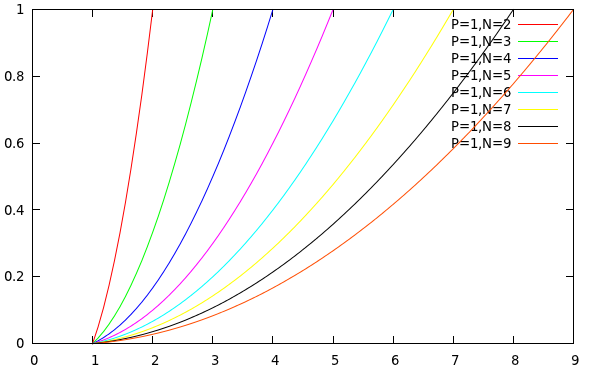
\includegraphics[width=\textwidth]{../../Graphics/AsyncCollusionSuccessFloor.png}

\section{Lemma: For any protocol where all players are rational and communication is asynchronous, rational coalitions have a greater than $\epsilon > 0$ chance of learning the secret before they would without collusion}

Let $n$ be the number of players.
Let $C$ be a rational coalition of players, selected randomly, with size less than the threshold $t$.
Let $r$ be the first round where a player would learn the secret if there were no collusion.
Let $L$ be the set of learners: players who learn the secret in round $r$.
Let $s$ be the sender of round $r$'s message.

The sender can not be one of the learners because the sender is receiving no new information during round $r$.

If the sender and at least one of the learners are in the coalition, then the coalition can internally simulate sending round $r$'s message before round $r$ occurs and thereby pre-emptively learn the secret. The probability of this occuring is $\frac{|C|}{n}*\frac{{n - |C| \choose |L|}}{{n - 1 \choose |L|}}$. This function varies with $L$, which the protocol has some control over. Higher values of $L$ give higher probabilities, so a lower bound for any protocol is setting $L$ to its minimum value: 1. This gives a lower bound probability of $\frac{|C|*(|C| - 1)}{N*(N-1)}$, which is independent of the protocol.

Pre-emptively learning the secret allows the sender to defect instead of cooperating in round $r$, lowering the probability of non-colluding players learning the secret. All asynchronous protocols are necessarily vulnerable to this type of internal-messaging attack. They may do worse, but they can't do better than defeating $\frac{|C|*(|C| - 1)}{N*(N-1)}$ of the coalitions of size $C$.

\section{Asynchronous Protocol for Inconspicuous Secrets and Bounded Opponents}

\subsection{Overview}

Each round $r$ the $r mod i$'th player sends a message created by a VRF provided by the dealer. The messages are added to offsets, also provided by the dealer, to create round shares. Before the target round the round shares are random gibberish, but the dealer chooses the offsets such that after the target round the round shares form a valid $t-1$ of $n$ set of shares for the secret (in an underlying secret sharing scheme like Shamir's). Players recognize the secret by a new round share being consistant with the previous $t-1$. $p$ should be set large enough to prevent the chance of this from happening accidentally. Players who recognize the secret will either defect or irrationally cooperate. If any of them irrationally cooperate, they will allow all other players to recognize the secret. Otherwise they will all defect, which indicates to the remaining players that the secret has been recognized.

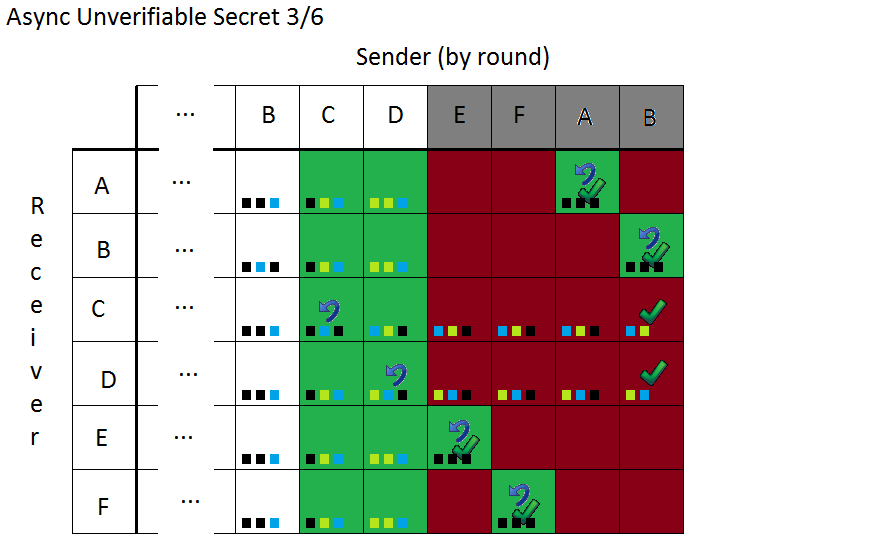
\includegraphics[width=\textwidth]{../../Graphics/AsyncInconspicuous_n6m3.png}

\subsection{Dealer Protocol}
\begin{itemize}
  \item Choose the protocol's parameters
    \subitem A prime $p$ larger than the largest possible secret
    \subitem The number of players $n$
    \subitem The threshold $t$
    \subitem The marginal probability of termination $\lambda$
    \subitem The VRF scheme
  \item Pick the secret $s$
  \item Create a VRF key pair $g_i, v_i$ for each player
  \item Generate $t-1 of n$ shamir shares $s_i$ in the finite field $Z_p$ for the secret 
  \item Pick a geometric-distributed round $r$ to be the target round
  \item Compute the secret-share/message offset $f_i$ for each player
    \subitem $f_i = s_i - VRF(g_i, r+i)$
  \item Send each player their generator
  \item Broadcast to every player the secret mask, prng seed, player verifiers and share masks
\end{itemize}

\subsection{Player Protocol}
\begin{itemize}
  \item For each round $r$
  \item Compute the potential secret $s$ using the $t-1$ preceeding round secret shares
    \subitem $s_{i mod n} = m_i + f_{i mod n}$
  \item If $r mod n = YourIndex$ then it is your turn to send
    \subitem Fail with no secret if there are fewer than $t$ players remaining
    \subitem Send $m_r, proof_r = VRF(g_i, r)$
  	\subitem Succeed with the potential secret if all other players defect
  \item Else
    \subitem Succeed with the potential secret if it is not changed by the new round share
  \item Continue to the next round if have not succeeded or failed 
\end{itemize}

\subsection{Strengths}

Malicious coalitions with at most $n-t$ members can't prevent the remaining players from learning the secret, because of the message verification. Their probability of success can be made exponentially small by increasing the strength of the VRF scheme. However, larger coalitions have other options. 

If there are at least $t$ non-colluding rational players then all rational players will learn the secret. A non-colluding rational player can either defect or cooperate. If they know the current potential secret is the true secret then they are expected to send no message. If they did send a message, it would only help the other players more. Once they know the secret, they can't defect. If they don't know the secret then there is a $\lambda$ chance the current potential secret is the true secret. Thus defecting will succeed with probability $\lambda$. But cooperating succeeds with at probability greater than $\lambda$, because the next message can show that the current potential secret is not the true secret. Therefore players are either incapable of defecting or do better by cooperating, meaning non-colluding rational players will cooperate. having at least $t$ cooperating players ensures they learn the secret so $t$ or more non-colluding rational players will learn the secret.

\subsection{Weaknesses}

Rational coalitions can pre-emptively learn the secret. If the player ordering places $c$ colluders at or past the $t-c$'th position then the coalition will learn the secret $c-1$ rounds earlier than any non-colluding rational player. This probability is bounded from below by $1 - \frac{{t - 1 \choose |C|}}{{n \choose |C|}}$, the probability of all colluders being placed at or past the $t-1$'th position. This lower bound gets worse as $n$ increasing, meaning there is a gap between the lower bound proven earlier to apply to all protocols ($\frac{|C|*(|C|-1)}{n*(n-1)}$) and the achieved bound. One or the other or both can be improved.

Coalitions of size $t-1$ can precompute all the potential secrets. This gives them a geometric distribution of possible secrets with significantly lower entropy, for reasonable values of $\lambda$, than the uniform distribution of possible secrets. Preventing this problem requires increasing $\lambda$ to increase the amount of entropy in the distribution, which increases the expected number of rounds.

When the number of cooperating players goes from $t$ to $t-1$, one of the remaining players will mistakenly accept a random secret as the true secret. This occurs because players stop cooperating when they realize fewer than $t$ players remain. The first player to notice will see $t-1$ players remaining, the second player will see $t-2$ remaining, and so forth until the last player to notice sees only themselves remaining. But this causes them to believe the other players disconnected due to the potential secret being the true secret, and so they accept whatever the potential secret happens to be as the true secret. Malicious coalitions with more than $n-t$ players can cause this scenario at will.

\chapter{Asynchronous Protocol for Conspicuous Secrets and Bounded Opponents}

The asynchronous protocol for inconspicuous secrets relied on the secret's inconspicuousness to allow the final $t-1$ senders to learn the secret. Even though they knew the most likely secret, they couldn't check it. When the secret is conspicuous, we can't rely on this property and must sacrifice one of the players.

\section{Overview}

This protocol is derived from the synchronous bounded protocol. The main difference is that the target round occurs at different times for different players, staggering their completion. 
 
\begin{figure}
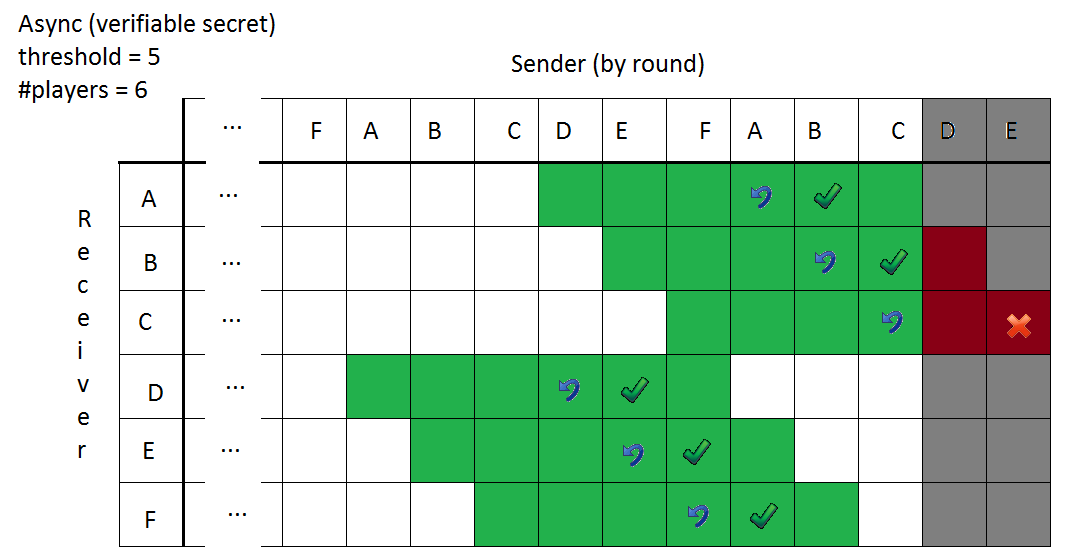
\includegraphics[width=\textwidth]{../../Graphics/AsyncVerifiedSecret_n6m5.png}
\caption{Asynchronous protocol for verifiable secrets with n=6, m=5. A player is sacrificed.}
\label{AsyncExample1}
\end{figure}

The proposed algorithm is basically a generalization of the synchronous algorithm. The main differences are that every player gets a different set of underlying secret shares to reveal, and they receive those shares on different rounds. Staggering the target rounds allows more players to stay in the dark about the game finishing until they have sent their message.

Example graphics (improve and add legends)

\section{Dealer Protocol}
\begin{itemize}
  \item Choose the protocol's parameters
    \subitem A prime $p$ larger than the largest possible secret
    \subitem The number of players $n$
    \subitem The threshold $t$
    \subitem The marginal probability of termination $\lambda$
    \subitem The VRF scheme
  \item Create a commitment to the secret
  \item Create a generator/verifier pair for each player
  \item Pick a geometric-distributed round to be the target round where the last shares are revealed
  \item Generate secret shares for the secret for each player, using any existing secret sharing scheme (e.g. shamir)
    \subitem The final round should have as many players broadcasting useful shares as possible.
    \subitem You can adjust when a player's first useful share is between 0 and M-2 before their turn.
    \subitem High precedence resists malicious players and avoids losers.
    \subitem Low precedence resists rational coalitions.
  \item Compute the share masks for each player pair
  \item Send each player their generator and share masks
  \item Broadcast to every player the commitment and all verifiers
\end{itemize}
\section{Player Protocol}
\begin{itemize}
	\item If you are sending this round, broadcast this round's generated value to all players
	  \subitem maskedShareMessage = Generator(round)
	\item Verify masked shares received from other players using their verifiers
	  \subitem Exclude players from future rounds if they send nothing when expected to send or send invalid potential shares
	\item Unmask the shares to reveal potential underlying shares and compute the potential secret
	  \subitem unmaskedShare(p) = maskedShareMessage(p) xor shareMask(p)
	  \subitem potentialSecret = combine(unmaskedShares)
	\item Stay for next round if the potential secret doesn't match the commitment
	\item Otherwise you have learned the secret and exit
\end{itemize}

\chapter{future work}

The synchronous protocol uses O(N) common share information and O(N) work per round. Can this be reduced to O(M) without sacrificing?

The asynchronous protocols have several areas where improvement is possible. The difference between the lower bounds and the achieved bounds is non-zero.

Is there a way to generate valid shares each round from independent seeds instead of having to generate random shares and targeting a single round? Would make things more convenient.

What are the effects of partial synchronization?

Losing all-receive-same?

\chapter{Conclusion}

\section{Summary}

\begin{tabular}{|r|r|r|}
\hline
							& Synchronous 					& Asynchronous\\
\hline
Conspicuous					& Optimal						& Sacrifical player, coalitions may succeed\\
Inconspicuous				& Make Conspicuous				& Coalitions may succeed\\
Inconspicuous + Unbounded	& ???							& Future work\\
\hline
\end{tabular}
\begin{tabular}{|r|r|r|}
\hline
Active & Synchronous & Conspicuous\\
\hline
Yes	& *		& *		\\
\multicolumn{3}{|l|}{Algorithm: Vote to Reveal}\\
\multicolumn{3}{|l|}{O(1) per-player secret shares (vote token)}\\
\multicolumn{3}{|l|}{O(1) all-player information (existence of secret)}\\
\multicolumn{3}{|l|}{Extendable without interaction}\\
\multicolumn{3}{|l|}{Rationals become honest}\\
\multicolumn{3}{|l|}{Irrationals drop}\\
\multicolumn{3}{|l|}{Rational coalitions offer no benefit, even beyond $M$}\\
\multicolumn{3}{|l|}{Irrational coalitions offer no benefit until $N-M+1$}\\
\multicolumn{3}{|l|}{Dealer dishonesty is detectable, assuming public messages?}\\
\hline
No	& Yes	& No \\
\multicolumn{3}{|l|}{Add conspicuousness without loss}\\
\hline
No	& Yes	& Yes \\
\multicolumn{3}{|l|}{Algorithm: Masks}\\
\multicolumn{3}{|l|}{O(1) per-player secret shares (key pair)}\\
\multicolumn{3}{|l|}{O(N) all-player information (masks, public keys)}\\
\multicolumn{3}{|l|}{Extendable with proxy interaction}\\
\multicolumn{3}{|l|}{Rationals become honest}\\
\multicolumn{3}{|l|}{Irrationals drop}\\
\multicolumn{3}{|l|}{Rational coalitions offer no benefit until $M$}\\
\multicolumn{3}{|l|}{Irrational coalitions offer no benefit until $N-M+1$}\\
\multicolumn{3}{|l|}{Dishonest dealer can undetectably deny service}\\
\hline
No	& No	& Yes	\\
\multicolumn{3}{|l|}{Algorithm: Staggered Masks}\\
\multicolumn{3}{|l|}{O(N) per-player secret shares (key pair, masks)}\\
\multicolumn{3}{|l|}{O(N) all-player information (public keys)}\\
\multicolumn{3}{|l|}{When all rational, 1 player doesn't learn the secret}\\
\multicolumn{3}{|l|}{Rational coalitions offer growing probabilistic benefit}\\
\multicolumn{3}{|l|}{Irrational coalitions \ldots ?}\\
\multicolumn{3}{|l|}{Dishonest dealer can undetectably deny service}\\
\multicolumn{3}{|l|}{Dishonest dealer can choose loser, assuming no irrationals}\\
\hline
No	& No	& No	\\
\multicolumn{3}{|l|}{Algorithm: Designed Transfers or maybe Masks+Rounds}\\
\multicolumn{3}{|l|}{O(R/N) per-player shares (messages)}\\
\multicolumn{3}{|l|}{O(N) all-player information (public keys)}\\
\multicolumn{3}{|l|}{1 player loses if there may be irrationals, otherwise use not send as eg. 'last message was secret'}\\
\hline
\end{tabular}

\chapter{Appendix - List of Definitions}

\begin{itemize}
  \item 'Efficient': A computation is efficient if it can be done in a practical amount of time. Essentially corresponds to polynomial time with respect to the input/key sizes. For fixed-size cases, seconds=efficient, centuries=inefficient is a reasonable rule of thumb.
  \item Knows: Can efficiently compute. If you know the prime factors then you know the product.
  \item Learns: Efficiently computes. Quick sort learns the sorted list.
\end{itemize}

\chapter{References}
\begin{thebibliography}{9}

\bibitem{} Rational Secret Sharing and Multiparty Computation

\bibitem{shamir} How to share a secret

\bibitem{} Games For Exchanging Information

\bibitem{} Collusion Free Protocol for Rational Secret Sharing

\bibitem{} Fairness with an Honest Minority

\bibitem{} Non-cooperative computation Boolean functions

\bibitem{} Rational Secret Sharing with Repeated Games

\bibitem{} The Deterministic Protocol for Rational Secret Sharing

\end{thebibliography}
\end{document}
